% document formatting
\documentclass[10pt]{article}
\usepackage[utf8]{inputenc}
\usepackage[left=1in,right=1in,top=1in,bottom=1in]{geometry}
\usepackage[T1]{fontenc}
\usepackage{xcolor}

% math symbols, etc.
\usepackage{amsmath, amsfonts, amssymb, amsthm}

% lists
\usepackage{enumerate}

% images
\usepackage{graphicx} % for images

% code blocks
\usepackage{minted, listings} 

% verbatim greek
\usepackage{alphabeta}

\graphicspath{{./assets/images}}

\newcommand{\solution}{\textbf{Solution:}} 

\title{COM SCI M151B Week 5}

\author{Aidan Jan}
\date{\today}

\begin{document}
\maketitle

\section*{Out of Order Execution}
\subsection*{Tradeoffs of Superscalar}
Advantages:
\begin{itemize}
    \item Higher IPC (instructions per cycle)
\end{itemize}
Disadvantages:
\begin{itemize}
    \item Higher complexity for dependency checking
    \item More hardware resources needed
\end{itemize}
Pipeline is typically never \textbf{full} due to frequent dependency stalls!
\subsection*{Summary}
\begin{itemize}
    \item Scalar processors are limited (i.e., best case: IPC=1)
    \item ILP and superscalar could provide this opportunity to parallelize data processing and achieve IPC > 1.
    \item In-order fetching prevents us from achieving the full potential of superscalar \textit{since usually there are not \textbf{enough} independent instructions in the pipeline.} 
    \item A solution is out-of-order execution!
\end{itemize}

\subsection*{Status Quo}
\begin{itemize}
    \item Superscalar (N = 2 or 4) with pipelining and forwarding and branch prediction!
    \item Ideally, we can get IPC=N with small CT
    \item Minimal overhead due to RAW data hazard (due to load-use)
    \item Minimal stall due to >90\% accuracy in branch prediction with only one cycle in miss penalty!
    \item Bottleneck
    \begin{itemize}
        \item Not all the pipeline lanes can be always utilized due to \textit{dependencies} and \textit{hazards}!
        \item Compilers can help but only in a limited form!
    \end{itemize}
    \item Instead of always executing the next instruction, why don't we find the first available instruction and feed that into the pipeline?
    \begin{itemize}
        \item If this instruction window is large enough, then we can always fully utilize our pipeline $\rightarrow$ IPC = N.
    \end{itemize}
\end{itemize}

\subsection*{How to execute instructions out-of-order}
\begin{itemize}
    \item A mechanism for \textit{tracking} instructions
    \begin{itemize}
        \item Later instructions might be \textbf{ready}.
    \end{itemize}
    \item A mechanism for \textit{removing} data hazards
    \begin{itemize}
        \item New hazards: WAW, WAR, load-store
    \end{itemize}
    \item A mechanism for \textit{recovery}
    \begin{itemize}
        \item Speculation (e.g., branch misprediction), etc.
    \end{itemize}
\end{itemize}

\subsection*{Out of Order Design}
\begin{center}
    \includegraphics*[scale=0.8]{W5_1.png}
\end{center}

\subsection*{Out or Order - Pipeline Recovery}
\begin{itemize}
    \item We need a temporary phase for some instructions so that if they need to be flushed, they can be easily erased!
    \begin{itemize}
        \item We define a new stage called "retire" (aka. "commit") and separate \textit{completion} from \textit{retire}.
    \end{itemize}
\end{itemize}

\subsection*{"Retire"/"Commit"}
What does it mean for an instruction to finish?
\begin{itemize}
    \item Writing back data to the register file, or
    \item Writing data to the memory, or
    \item Updating the PC (branch)
\end{itemize}
If the data is already writtenm it is too late to flush, thus we should write somewhere temporarily until we are certain!

\subsection*{Complete vs. Retire}
\begin{itemize}
    \item Idea: to enable recovery, allow instructions to complete (i.e., prepare the final result) out of order, but retire them (i.e., actually writing data permanently) in order.
    \item We call writing data permanently, writing to architectural state (i.e., registers/memory)
\end{itemize}

\subsection*{How to Implement retire?}
\begin{itemize}
    \item Need a buffer/storage to store temporary data!
    \item Need a mechanism to follow instructions in order and out of order to find out when to retire!
\end{itemize}

\subsection*{How to "retire" in-order?}
\begin{itemize}
    \item Re-order buffer (ROB)
    \begin{itemize}
        \item ROB is a (circular) table/buffer that holds \textbf{completed} instructions.
        \item ROB requires an instruction $I_x$ only if \textit{all} $I_j$ (for $j < x$) are retired.
    \end{itemize}
\end{itemize}
Datapath with ROB:
\begin{center}
    \includegraphics*[scale=0.8]{W5_2}
\end{center}

\subsection{What if we start executing out of order?}
Examples:
\begin{itemize}
    \item RAW (Read After Write) = "true dependence"
    \begin{verbatim}
        add x2, x1, x3              sub x4, x3, x2    
        ...                 -->     ...
        sub x4, x3, x2              add x2, x1, x3
    \end{verbatim}
    \item WAW (Write After Write) = "output dependence"
    \begin{verbatim}
        add x2, x1, x3              sub x2, x3, x4
        ...                 -->     ...
        sub x2, x3, x4              add x2, x1, x3
    \end{verbatim}
    \item WAR (Write After Read) = "anti-dependence"
    \begin{verbatim}
        add x3, x1, x2              sub x2, x3, x4
        ...                 -->     ...
        sub x2, x3, x4              add x3, x1, x2
    \end{verbatim}
\end{itemize}
The WAW and WAR are called "False Dependencies".  These can be fixed by simply changing the register, e.g., changing the \texttt{x2} in the sub instructions to \texttt{x5} instead.\\
The RAW case is the true dependence, and in that case, the solution is much more complex.  We will discuss this later!

\subsection*{Register Renaming}
\begin{itemize}
    \item The problem is that we have \textbf{limited architectural registers} (ISA registers, e.g., 32 in RISC-V)
    \item However, we can have much more \textbf{physical} registers (e.g., 128 registers).
    \item One architectural register (A-reg) can be assigned to \textbf{multiple physical registers} (P-reg).
\end{itemize}
\subsubsection*{How to do renaming?}
\begin{itemize}
    \item Register Alias/Map Table (RAT)
    \begin{itemize}
        \item One entry per architectural register.
        \item Each entry stores the \textit{physical location of the most recent} version of the architectural (logical) register.
        \item \textbf{Algorithm:}
        \begin{itemize}
            \item For each \underline{destination} A-reg, the renaming algorithm assigns a new P-reg from a \textit{pool of free (physical) registers}.
            \item For each \underline{source} A-reg, the renaming algorithm accesses RAT and finds the corresponding P-reg.
        \end{itemize}
    \end{itemize}
\end{itemize}

\subsubsection*{Renaming Example}
\begin{itemize}
    \item Let's assume that
    \begin{itemize}
        \item We have 5 architectural registers and 10 physical registers.
        \item The \textit{initial} mapping looks like this:
        \begin{center}
            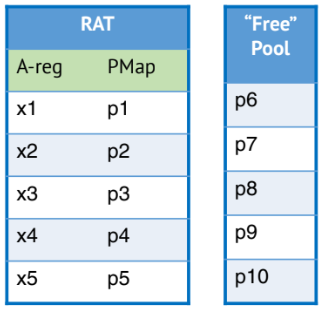
\includegraphics[scale=0.9]{W5_3.png}
        \end{center}
    \end{itemize}
    \item Consider the instructions:
    \begin{verbatim}
        or x3, x2, x1
        add x4, x3, x4
        sub x3, x5, x2
        addi x1, x3, 2
    \end{verbatim}
    \item Following the RAT, we get:
    \begin{verbatim}
        or x3, x2, x1       --> or p6, p2, p1
        add x4, x3, x4
        sub x3, x5, x2
        addi x1, x3, 2
    \end{verbatim}
    \item We assign x3 to point to p6 instead of p3
    \begin{center}
        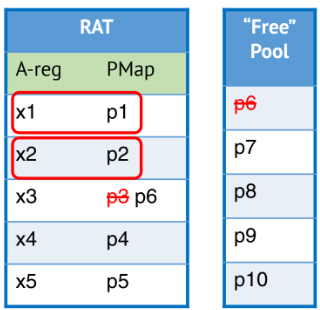
\includegraphics[scale=0.9]{W5_4.png}
    \end{center}
    \item Now, we fill the second line:
    \begin{verbatim}
        or x3, x2, x1       --> or p6, p2, p1
        add x4, x3, x4      --> add p7, p6, p4
        sub x3, x5, x2
        addi x1, x3, 2
    \end{verbatim}
    \item Now, in this step, we assign x4 to p7.
    \begin{center}
        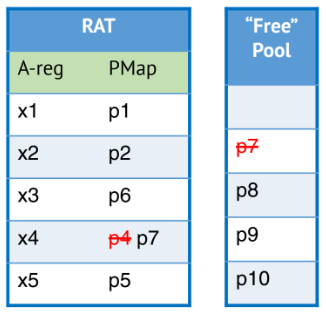
\includegraphics[scale=0.9]{W5_5.png}
    \end{center}
    \item Et cetera, we do reassignments for the destination registers.
    \begin{verbatim}
        or x3, x2, x1       --> or p6, p2, p1
        add x4, x3, x4      --> add p7, p6, p4
        sub x3, x5, x2      --> sub p8, p5, p2
        addi x1, x3, 2      --> addi p9, p8, 2
    \end{verbatim}
    \begin{center}
        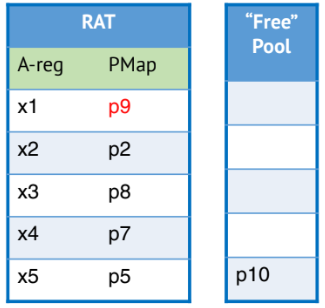
\includegraphics[scale=0.9]{W5_6.png}
    \end{center}
\end{itemize}
\subsubsection*{When to free?}
We free the previous, "old" destination register when the instruction is retired.  e.g., once the first instruction is executed (and retired), we can free p3 (not p6!), because that means that the value of p3 is no longer used since it got reassigned.
\subsubsection*{Datapath with Renaming and ROB}
\begin{center}
    \includegraphics*[scale=0.7]{W5_7.png}
\end{center}    
\subsection*{Recap}
At this point, we have the mechanism for removing data hazards and the mechanism for recovery.\\\\
Now, we just need the mechanism for \textit{tracking} instructions, as described earlier.

\subsection*{How to Schedule}
\begin{itemize}
    \item We need a mechanism to track who is ready:
    \begin{itemize}
        \item \texttt{I3} is not ready, but \texttt{I4} is!
        \item Who is ready?
        \begin{itemize}
            \item This also helps to fix RAW hazards (i.e., forwarding!)
        \end{itemize}
    \end{itemize}
\end{itemize}

\subsection*{Reservation Station}
\begin{center}
    \includegraphics*[scale=0.8]{W5_8.png}
\end{center}
Now, we can remove the MEM stage and consolidate it to one \textbf{functional unit,} with multiple units (FUs)
\begin{center}
    \includegraphics*[scale=0.8]{W5_9.png}
\end{center}
Our pipeline looks like this:
\begin{center}
    \includegraphics*[scale=0.8]{W5_10}
\end{center}
\subsection*{Steps}
\begin{enumerate}
    \item Fetch
    \item Dispatch: putting instructions in reservation station.
    \begin{itemize}
        \item Copying values (e.g., rsl) to RS.
        \item Reserving an entry in ROB
        \item If RS or ROB is full, stall the backend.
    \end{itemize}
    \item Issue/Fire: starting the execution once all sources are ready and the FU is available.
    \begin{itemize}
        \item Releasing the entry in RS (but not ROB).
    \end{itemize}
    \item Complete: copying results to the ROB.
    \begin{itemize}
        \item Releasing FU.
        \item Mark Rd \textit{ready} $\rightarrow$ forwarding happens here!
    \end{itemize}
    \item Commit/Retire: writing the results to architectural state (i.e., register and memory)
    \begin{itemize}
        \item If this instruction is the top of ROB, commit.
        \item Mark old (physical) register as free.
    \end{itemize}
\end{enumerate}

\subsection*{Out of Order Execution Example}
\begin{center}
\includegraphics*[width=\textwidth]{W5_out_of_order/0.png}\\
\includegraphics*[width=\textwidth]{W5_out_of_order/1.png}\\
\includegraphics*[width=\textwidth]{W5_out_of_order/2.png}\\
\includegraphics*[width=\textwidth]{W5_out_of_order/3.png}\\
\includegraphics*[width=\textwidth]{W5_out_of_order/4.png}\\
\includegraphics*[width=\textwidth]{W5_out_of_order/5.png}\\
\includegraphics*[width=\textwidth]{W5_out_of_order/6.png}\\
\includegraphics*[width=\textwidth]{W5_out_of_order/7.png}\\
\includegraphics*[width=\textwidth]{W5_out_of_order/8.png}\\
\includegraphics*[width=\textwidth]{W5_out_of_order/9.png}\\
\includegraphics*[width=\textwidth]{W5_out_of_order/10.png}\\
\includegraphics*[width=\textwidth]{W5_out_of_order/11.png}\\
\includegraphics*[width=\textwidth]{W5_out_of_order/12.png}\\
\includegraphics*[width=\textwidth]{W5_out_of_order/13.png}\\
\includegraphics*[width=\textwidth]{W5_out_of_order/14.png}\\
\includegraphics*[width=\textwidth]{W5_out_of_order/15.png}\\
\includegraphics*[width=\textwidth]{W5_out_of_order/16.png}\\
\includegraphics*[width=\textwidth]{W5_out_of_order/17.png}\\
\includegraphics*[width=\textwidth]{W5_out_of_order/18.png}\\
\includegraphics*[width=\textwidth]{W5_out_of_order/19.png}\\
\includegraphics*[width=\textwidth]{W5_out_of_order/20.png}\\
\includegraphics*[width=\textwidth]{W5_out_of_order/21.png}
\end{center}
\subsection*{Summary}
We now have a way to execute instructions out of order with the three parts discussed earlier:
\begin{itemize}
    \item A mechanism for \textit{tracking} instructions
    \begin{itemize}
        \item Later instructions might be \textbf{ready}
    \end{itemize}
    \item A mechanism for \textit{removing} data hazards
    \begin{itemize}
        \item \textbf{New} hazards: WAW, WAR, load-store
    \end{itemize}
    \item A mechanism for \textit{recovery}
    \begin{itemize}
        \item \textit{Speculation} (e.g., branch misprediction), etc.
    \end{itemize}
\end{itemize}
\subsection*{Datapath with ROB, RAT, FU}
\begin{center}
    \includegraphics*[scale=0.7]{W5_11.png}
\end{center}
\begin{itemize}
    \item Each unit can be further split into multiple stages (not shown here).
\end{itemize}
\end{document}



